\documentclass{article}
\usepackage[T1]{fontenc}
\usepackage{lmodern}
\usepackage{graphicx}
\usepackage{amsmath,amssymb}
\usepackage[a4paper,margin=2cm]{geometry}
\usepackage[absolute,overlay]{textpos}
\setlength{\TPHorizModule}{1mm}
\setlength{\TPVertModule}{1mm}
\usepackage[indonesian]{babel}
\usepackage{hyperref}
\setlength{\emergencystretch}{2em}
% unit: Halaman 62

\begin{document}

% === Halaman 62 (llm) ===

\section*{3. Fungsi Hash}

\begin{itemize}
    \item Mengkompresi pesan ukuran sembarang menjadi \textit{message-digest} berukuran \textit{fixed}.
    \item \textit{Irreversible} (tidak bisa dikembalikan menjadi pesan semula)
\end{itemize}

\vspace{10mm}

\begin{itemize}
    \item MD5
    \item SHA-1
    \item SHA-2
    \item Keccak (SHA-3)
    \item RIPEMD
    \item WHIRLPOOL
\end{itemize}

% deskripsi: Diagram alur fungsi hash yang menunjukkan input (Masukan) diproses oleh 'Fungsi hash' untuk menghasilkan 'Nilai hash' berupa string heksadesimal, dengan tiga contoh input yang berbeda.
% bbox normalisasi: [0.1200, 0.3800, 0.6300, 0.9200]
\begin{textblock*}{107.10mm}(25.20mm,112.86mm)
\noindent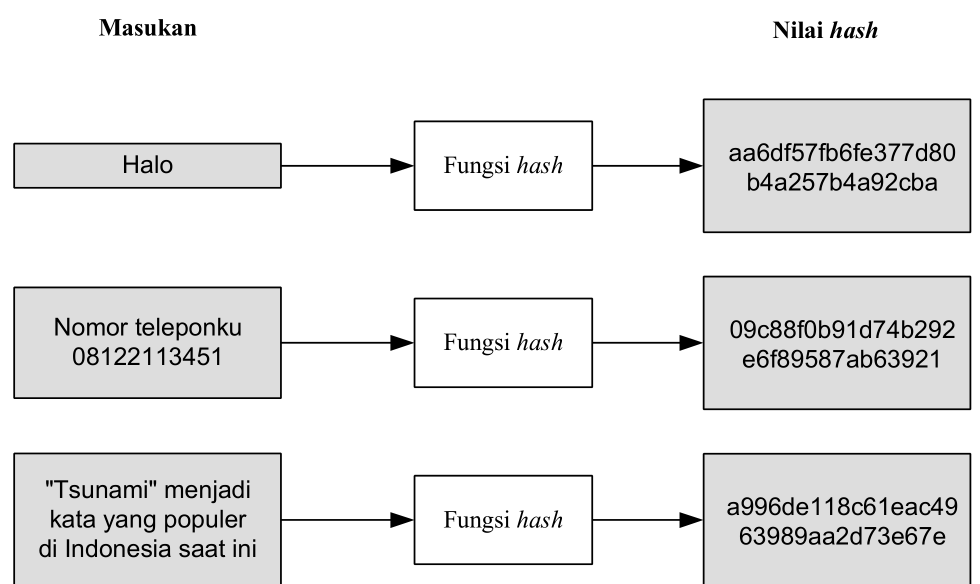
\includegraphics[width=107.10mm,height=160.38mm]{../../images/llm/page_062_img_01.png}%
\end{textblock*}

\end{document}
